% !TEX root=../thesis.tex

\begin{flushright}{\slshape 
	I would like to make a case for the car, despite all the manufacturers' 
	claims down the decades,\\
	being the piece of technology that has made the slowest advances 
	towards the clean, safe, digital,\\
	pastel-colored, technology-dominated, communications-driven future that 
	awaits us.\\
	It is still an analogue great lump of metal, a simple machine that we 
	must operate. \\
	Thank God.} \\ \medskip
		--- Richard Hammond \cite{Hammond} 
\end{flushright}


\bigskip

\begingroup
\let\clearpage\relax
\let\cleardoublepage\relax
\let\cleardoublepage\relax


\chapter{Background and State of The Art}

In this chapter we will discuss the background for the project and present 
related theory and research.
We will also spend some time on modern car electronics and sensor systems, and the state of the art for
In Vehicle Information Systems (IVIS) and display technology.
\\
\section{Revolve NTNU}
Revolve NTNU is a student organization which participates in the Formula 
Student competition. Founded in 2010 based on the wish to get more practical 
experience during their studies at NTNU. \cite{Revolve:history} Revolve has competed in Formula Student 
UK (FSUK) and Formula Student Germany (FSG) in both 2012 and 2013. The team is now 
well underway in designing the car for the 2014 competitions. See appendix
\vref{appendix:formula}
for more details about the Formula Student series of competitions.


\subsection{Entries}
The 2012 and 2013 contributions from Revolve both came in the form of a petrol powered race car driven by an internal combustion engine (ICE)
 \cite{Revolve:car13}.
The cars are built to comply with restrictions and demands posed by rules and 
regulations. These regulations set, among others, limits for size of the car, 
requirements for the driver position and power output.
The 2014 contribution, which at time of writing is in the design phase, is going to be a battery powered race car driven by an electric motor \cite{Revolve:car14}.

The choice of an electrically powered drive-train changes some aspects of the 
car compared to using an ICE. Most notably there's not going to be multiple 
selectable gear-ratios, 
but instead one fixed gear ratio. As for sensors and electronics there is not 
a very big change. There are however some changes in instrumentation;
there is no need to
let the driver know he should change gears for instance.  
On the other hand, there will be high density batteries which develops heat and need to be cooled, and there is also a need to inform the driver
of the battery charge level.

\section{Instrumentation and Control}


\subsection{Sensors and control networks}
Both racing  and  personal vehicles are fitted with complex mechanical and electrical
systems being controlled mostly by small embedded computers. For these systems
to be able to perform regulation they need input data about the state of
the surrounding and controlled systems. This data is gathered by means of
sensors registering real-world factors like position, temperature, pressure,
and flow that in turn is feed into the control system.

Sensor systems can also be used to gather data to create meaningful feedback 
for the driver or operator. This is usually visualized through the instruments
located in the dashboard, but can also be conveyed through other means (parking
sensors usually utilize sound).

\begin{figure}[!htbp]
	\includegraphics[width=\textwidth]{human-loopback-control.png}
	\caption{A sensor system where data is used to create feedback for the driver.}
	\label{fig:human-loopback}
\end{figure}

\begin{figure}[!htbp]
	\includegraphics[width=\textwidth]{simple-loopback-control.png}
	\caption{A simple loopback control system.}
	\label{fig:simple-loopback}
\end{figure}
\noindent Traditionally sensors used to be directly wired to the control unit (see \vref{fig:simple-loopback}), but as
system complexity and the
number of sensors grew this made the overall complexity very high. In addition
some sensors are very far away from their control units, examples are sensors 
that detect collisions and wheel speed. The solution to avoid having several 
kilometers of wires is to utilize digital communication buses which allows
components to communicate with each other and significantly reduces the amounts of 
wires needed. It also allows one sensor to input signals to multiple
control systems.
\begin{figure}[!htbp]
	\includegraphics[width=\textwidth]{intermediate-loopback-control.png}
	\caption{A message passing loopback control system. The control unit receives
	message through a sensor network.}
	\label{fig:intermediate-loopback}
\end{figure}

The most significant bus-standard is the Controller Area Network bus
(``CAN-bus'')
that was developed specifically to be used for automotive purposes and is
very error-resilient \cite[1]{can-appnote}.

In a CAN system connected nodes communicate by sending messages (``frames'').
Frames have an id which is also the priority of the message (lower number =
higher priority), if two nodes attempt to send at the same time the frame
with the highest priority will be transported over the bus, the losing node
will retry when the bus is clear. \cite{can-appnote}

The CAN standard is present in the majority of modern cars, which are (more or less) required to
have a CAN-bus through the OBD-II standard \cite{wiki:OBDII}. CAN is also seeing
great adoption in other areas as well. At NTNU CAN is the most emphasized
communication standard in the ``Industrial and Embedded Computer Systems
Design'' course, and is also, coincidentally, the communication standard 
Revolve has decided to
use in their designs. CAN-buses allows easy connection of components and is
also quite fault tolerant, which makes it very applicable for automobile
purposes \cite{can-appnote}.

ISO11898 and ISO11519 describe high- and low-speed interfaces for CAN. 
Together with the CAN-standard these provide the lower 
two layers of the OSI-model \cite{microsoft:osi}. The other layers are 
implementation specific; meaning that routines, package structure, 
and error handling routines are defined by the developers. This means that 
implementations are application specific, but also gives the 
developer room for utilizing the bus the way they see fit. \cite{can-appnote}

\subsection{Digital communication with analog sensors}
Output from a sensor doesn't necessarily make much sense if you view the raw data, 
for instance - a temperature sensor might give outputs between 0 and 5 volts.
Sensors are in their very nature analog\footnote{However digital sensors are
becoming more and more common, they do however still contain the same
components, the difference is that they are packaged together - reducing development
time and physical size of sensor assembly.} and thus requires their output
values to be represented digitally. Although some modern sensors come with
digital outputs, most sensors requires peripheral components that adapt an
output voltage to a level suitable for digitalizing before an analog-to-digital
converter reads the voltage and can communicate it to other digital components,
most commonly a micro controller unit (MCU). The MCU would then take the value
from the sensor, wrap it in a CAN-frame and transmit it on the
CAN-bus, either at its own accord or when requested from another node. \cite[loc. 5020-5203,
5732-7565]{catsoulis:embedded}\cite{can-appnote}
\begin{figure}[!htbp]
	\includegraphics[width=\textwidth]{simple-sensor-and-ad.png}
	\caption{Example of a modern sensor assembly. The sensors analog output is converted to a
	4-bit
	digital signal using an analog/digital converter, its output is read by a
	microcontroller and transmitted over a CAN-network with the use of a
	CAN-tranceiver. Blue lines indicates signal path.}
	\label{fig:simple-sensor}
\end{figure}


\subsection{Electrical noise and protection}
Wires are basically antennas and are susceptible to catching induced currents
from magnetic fields, and also emits their own magnetic fields when current is
applied. Petrol engines use high-voltage components that may create a lot of
noise if not shielded properly. This often results in noisy electrical
environments, something even modern cars struggle with. Automobile electronics
have to be designed to tolerate very high transient voltages. \cite[loc. 2562]{catsoulis:embedded}\footnote{loc. refers to Kindle location. This cannot be compared to ordinary page numbering.}

\subsection{Display Technology}
The standard information system for cars is obviously the dashboard, but it too
has undergone changes and in modern iterations are becoming increasingly
sophisticated. Mercedes have for some years been offering cars with night
vision cameras and a screen overlay in the dashboard \cite{Daimler}. BMW are
offering head-up displays on some of their models, claiming it allows drivers
to process information up to 50\% faster \cite{BMW}.

2012 saw the announcement of Google's ``Glass'' project \cite{nytimes:glass}, a set of smart-glasses
running a modified version of Android \cite{androidnews:glassAndroid}. It is not the
first example of such technology, but Google Glass did draw focus to the field.
Since then a lot of other projects have gotten traction; Optinvent,
who's been researching this type of technology for a long time, announced in 
2013 that they were planning to bring their own smart-glasses, ``ORA'', to the
market \cite{optinvent:press}. ORA has a color display and a bigger field-of-
view than Google Glass, and can be used for both augmented reality\footnote{
	Overlaying information about your surroundings onto them. 
} as well as 
a ``look-down'' screen \cite{optinvent:ora}. In late 2013 Nissan 
demonstrated a prototype wearable head-up unit, the
``3E'' \cite{caranddriver:nissan_3E}, which showcases telemetry data
visualization.

Motorcyclists have also been giving the idea of head-up displays a thought, and
except for the SportVue \cite{motionResearch:sportvue} which was criticized for
being overly difficult to install \cite{bikeland:sportvueDidntWork}, they are
all fairly new and mostly at the prototype stage
 \cite{skully,cycleworld:nuviz,popularscience:livemap}. The common point for
these is that (except for SportVue) they rely on GPS data and internal sensors
instead of telemetry data from the motorcycle itself.

Fighter planes have been utilizing head-up displays for over 40 years
 \cite{debellis1973flight}, and they have also turned to
helmet mounted displays to further enable the pilot \cite{barnes:tacticalHud}, but even today the
technology remains to be perfected \cite{independent:blindedPilot}.

\section{Software Architecture Patterns}
Software architecture can be seen as the bridge between business goals and the resulting
system \cite{bass2012software}. Both Larman \cite{Larman:UML} and Bass et al.
 \cite{bass2012software} suggest architectural design through applying known
patterns to common problems. In this section we will look at some patterns 
that are relevant for our system.

The \textit{model-view-controller} pattern is usually associated with
interactive software utilizing a graphical user interface, but can for 
instance be adopted to be used with web pages. The main strength is to use a
controller to manage transformations between a view and the data and 
application logic (model). One of the main benefits with the MVC-pattern is
loose coupling and the ability to easily create multiple views for a single
model. \cite[pp. 213-215]{bass2012software}
\begin{figure}[!htbp] %go figure :P
	\includegraphics[width=\textwidth/2,center]{model-view-controller.png}
	\caption{The model-view-controller-pattern. \cite[p. 214]{bass2012software}}
	\label{fig:mvc-pattern}
\end{figure}

\textit{Pipe-and-filter} is pattern that is well suited for transforming
multiple streams of data through a series of transformations. Multiple filters
can be connected together with pipes. This pattern is typically ill suited for
interactive systems or long running computations. A filter can have
multiple inputs and multiple outputs, a pipe has only one input and one output
and performs no transformations. \cite[215-217]{bass2012software}
\begin{figure}[!htbp] %go figure :P
	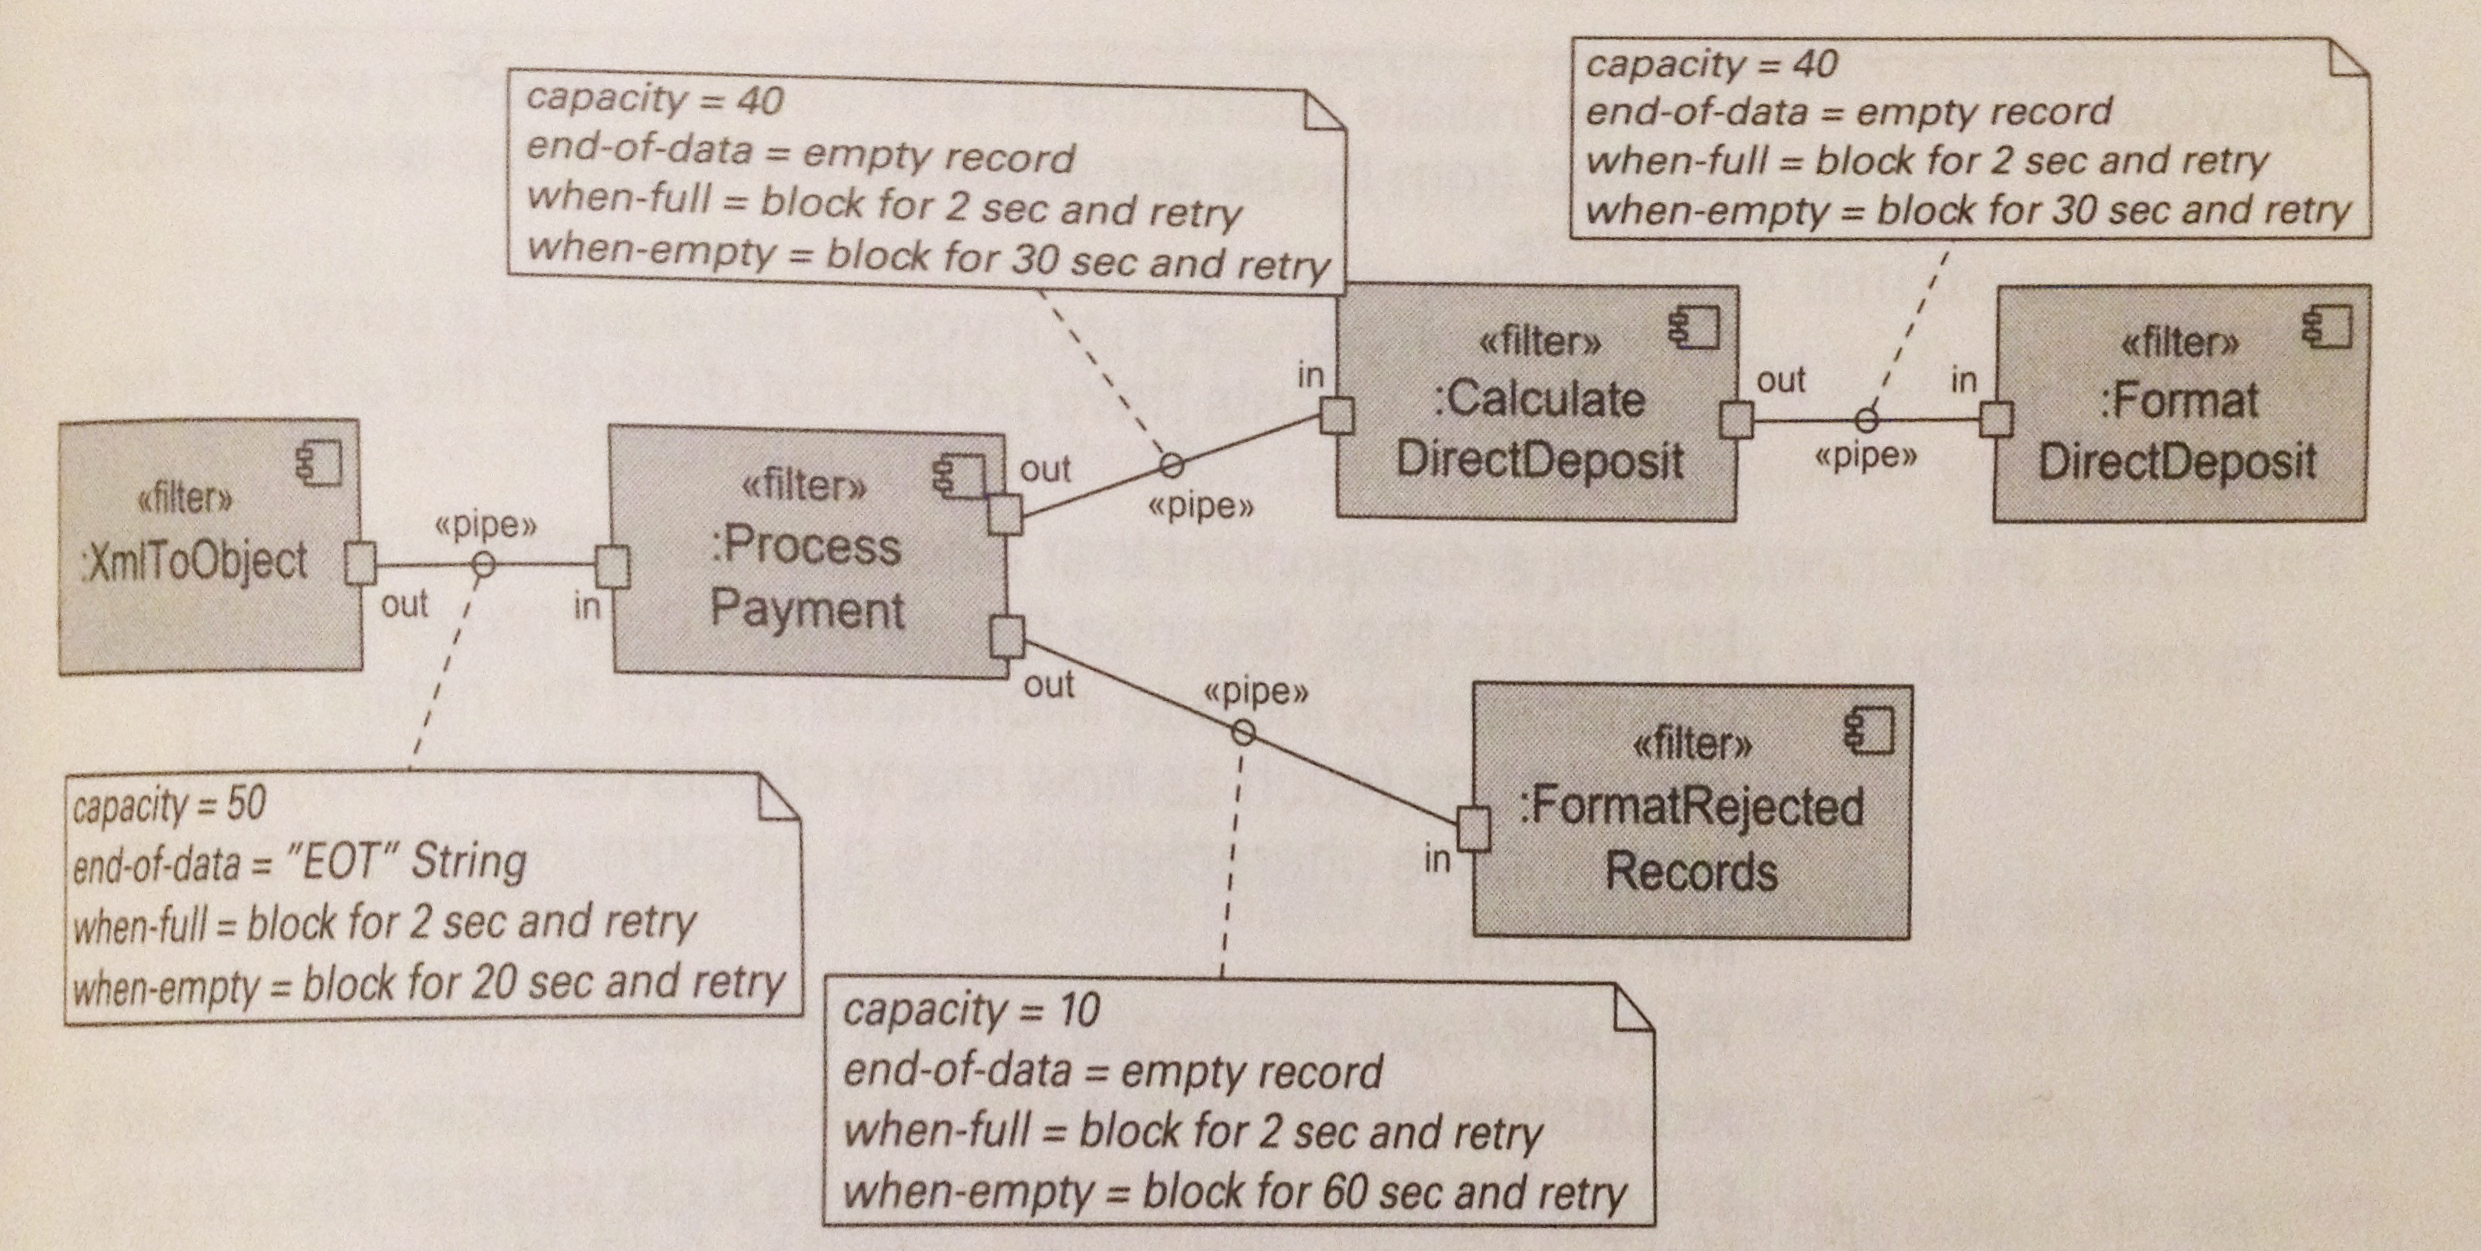
\includegraphics[width=\textwidth/2,center]{pipes-and-filters.png}
	\caption{The pipe-and-filter-pattern. \cite[p. 217]{bass2012software}}
	\label{fig:pipeandfilter-pattern}
\end{figure}

The \textit{layered} pattern is a way to provide a separations of concern
(segmentation between modules) in a complex system. This allows modules to be
developed and modified separately, without changing other modules. This relies
on principle that each layer provides a stable interface. Normally in a layer
architecture each layer can communicate only with the next (lower) layer. There
are however many violations to the pattern made for trade-off reasons, usually
performance. According to Bass et al.. it is one of the most commonly used 
patterns in software engineering. \cite[pp. 205-210]{bass2012software}

The \textit{multi-tier} pattern is often used to distribute a system into
distinct subsets. It is often used when different software components are
running on different physical nodes. Each tier represents a logical grouping of
components. One computing node can run multiple tiers, but still communicate
through a defined interface between the nodes. Tiering adds a level of
abstraction that introduces overhead and increases system complexity, but the
trade-offs include increased modifiability and reduces coupling.
 \cite[pp. 235-238]{bass2012software}

\section{Related Research}
\label{background:rel_reasearch}
The majority of research related to motorsport is related to design and
construction; very little research has been performed with the goal of giving
the driver a better environment. Most of the research done on driver
environments and IVIS is focused on safety. Lim et al. \cite{lim1999heads}
tested a prototype HUD-solution in a snow plow with focus on low visibility
conditions. Cheng et al. \cite{cheng2007intelligentVehicles} tested drivers
ability to follow the speed limit when aided by a HUD-display. A collision 
warning and traffic monitoring system was tested on military vehicles by
Nishizawa et al. \cite{nishizawa1997heads}, which in addition to a HUD also
used sounds to alert the driver. Cottle et al. \cite{wirelessDashboard}
designed a wireless ``dashboard'' built into a steering wheel in a Formula
Student car, but very little focus was put on the end user experience. There
has also been done some studies on the effect of distractions on driver response
time, both cognitive \cite{visualDistractionsStudy} and physical 
distractions \cite{hancock1999effects} have been studied.

Goeble et al. \cite{goebl2007realtimecapable}
developed an architecture that supported interchange of information with
different temporal resolution between computing nodes in cognitive automobiles.
The system is very large and complex and is made to support exchange of
information between multiple consumers and producers with either hard or soft 
real-time requirements.

Stewart et al. \cite{stewart1993integration} developed a framework that
utilized a global state table with a single lock to facilitate information 
exchange in reconfigurable sensor-based control systems. Although the paper is
from 1993 it is still relevant to our application, however the inter-component communication described is significantly
different from the serial buses utilized in modern cars.

In their 1995 paper Magee et al. \cite{magee1995specifying} presents the 
Darwin notation for specifying the architectural level of distributed 
systems. Darwin is an architecture description language (ADL), another ADL is
Wright \cite{Allen97Thesis}. ADLs are used to formally describe software architectures.
Despite their common goals, Allen \cite[p. 24]{Allen97Thesis} argues that Darwin
``does not provide an adequate basis for analysis of the behavior of an
architecture.''.



\endgroup %Resets chapter page-shifting before next chapter :)
